% !TEX TS-program = lualatex

% required for TexXstudio, an alternative is to change the default bibliography tool 
% in TeXstudio settings (Options > Configure TeXstudio > Build > Default Bibliography Tool)
% !BIB TS-program = biber

\documentclass[a4paper,11pt]{article}

\usepackage{geometry}
\geometry{left=20.00mm, right=15.00mm, top=20.00mm, bottom=20.00mm}

% this is to get rid of 'Overfull \hbox...' errors
\usepackage{microtype}

% ------------------------------------------------------------------------------
% Title
% ------------------------------------------------------------------------------

\title{\vspace{-1.5cm}Математический анализ и линейная алгебра \\
Домашнее задание №2}
\author{Дмитрий Донецков (ddonetskov@gmail.com)}
\date{\today}

% ------------------------------------------------------------------------------
% LUA
% ------------------------------------------------------------------------------

% \usepackage{luacode}

% ------------------------------------------------------------------------------
% Graphics
% ------------------------------------------------------------------------------

\usepackage{graphicx}

% https://www.sharelatex.com/learn/Pgfplots_package
\usepackage{pgfplots}
\pgfplotsset{compat=1.15}\usepgfplotslibrary{fillbetween}

\usepackage{wrapfig}

% ------------------------------------------------------------------------------
% Figures
% ------------------------------------------------------------------------------

\usepackage{subcaption}         % subcaptions in figures

% ------------------------------------------------------------------------------
% Tables
% ------------------------------------------------------------------------------

\usepackage{multirow}           % spanning columns across multiple rows
\usepackage{makecell}           % allows different formats inside cells

\renewcommand\theadalign{bc}
\renewcommand\theadfont{\bfseries}
\renewcommand\theadgape{\Gape[4pt]}
\renewcommand\cellgape{\Gape[4pt]}

% ------------------------------------------------------------------------------
% Math (Additional Support)
% ------------------------------------------------------------------------------

\usepackage{amsmath,amsfonts,amssymb,amsthm,mathtools}     % AMS
\usepackage{cancel}             % four different modes of striking through
\usepackage{dsfont}
\usepackage{icomma}             % Smart comma: $0,2$ --- число, $0, 2$ --- перечисление
%\usepackage{nicefrac}          % looks like xfrac is better maintained
\usepackage{physics}            % implementation of \abs and \norm
\usepackage{xfrac}

\DeclareMathOperator*{\D}{\mathbb{D}}   % the dispersion symbol
\DeclareMathOperator*{\E}{\mathbb{E}}   % the expectation symbol

\DeclareMathOperator*{\N}{\mathbb{N}}   % the set of natural numbers
\DeclareMathOperator*{\R}{\mathbb{R}}   % the set of real numbers
\DeclareMathOperator*{\Z}{\mathbb{Z}}   % the set of integers

% e = 2.71...
\newcommand{\e}{\mathrm{e}}

% sign of independence
% \vDash can also be used instead of \models
% \raisebox{}{} is required for vertical alignment
\newcommand{\independent}{\raisebox{0.05em}{\rotatebox[origin=c]{90}{$\models$}}}

%\newcommand\independent{\protect\mathpalette{\protect\independenT}{\perp}}
%\def\independenT#1#2{\mathrel{\rlap{$#1#2$}\mkern2mu{#1#2}}}

% ------------------------------------------------------------------------------
% Russian Language (support thereof)
% ------------------------------------------------------------------------------

\usepackage[russian,english]{babel}	    % локализация и переносы

% ------------------------------------------------------------------------------
% Fonts 
% ------------------------------------------------------------------------------

\usepackage{fontspec}           % required to load Open Type, True Type fonts

\setmainfont{CMU Serif}
\setsansfont{CMU Sans Serif}
\setmonofont{CMU Typewriter Text}

%\setmainfont{Linux Libertine O} % Libertine covers Latin, Hebrew, Greek, and Russian
%\setmonofont{Courier New}

\usepackage{euscript}	          % Шрифт Евклид
\usepackage{mathrsfs}           % Красивый матшрифт

% ------------------------------------------------------------------------------
% Bibliography 
% ------------------------------------------------------------------------------

% Removed as it was not required.

% ------------------------------------------------------------------------------
% Bookmarking, citing, URL's
% ------------------------------------------------------------------------------

% hyperref usually needs to be loaded last
\usepackage{hyperref}
\usepackage{url}
% \usepackage[dvipsnames]{xcolor}

\hypersetup{
    colorlinks=true,
    linkcolor=blue,
    filecolor=red,      
    urlcolor=blue,
}

\urlstyle{same}

% ------------------------------------------------------------------------------
% Various
% ------------------------------------------------------------------------------
\usepackage{listings}
\lstset{showstringspaces=false}



\begin{document}

\maketitle

\section{Задачи}

\subsection{Задача 1}

a) Согласно определению $O(g(x))$ проверим выполняется ли условие

\begin{align}
\label{eq:t1a1}
\bigg\lvert \frac{x^2 + 3}{x - 4} \bigg\rvert < C|x|, x \rightarrow \infty.
\end{align}

Для чего приведём неравенство в такой вид, чтобы его можно было легко проверить:

\begin{align}
\label{eq:t1a2}
\frac{x^2 + 3}{x - 4} & = \frac{(x-4)(x+4) + 19}{x - 4} = (x+4) + \frac{19}{x-4}
\end{align}

Подставим получившееся выражение \ref{eq:t1a2} в неравенство \ref{eq:t1a1}.

\begin{align*}
|(x+4) + \frac{19}{x-4}| < C|x| 
\quad \Rightarrow \quad 
|1 + \frac{4}{x} + \frac{19}{x(x-4)}| < C, \quad x \rightarrow \infty
\end{align*}

Левая часть неравенства при $x \rightarrow \infty$ стремится к 1, что меньше константы $C$, соответственно, исходное утверждение - верное.

\bigskip

б) Согласно определению $O(g(x))$ проверим выполняется ли условие

\begin{align*}
\bigg\lvert \frac{x^2 + 3}{x - 4} \sin x \bigg\rvert < C|x^k|, x \rightarrow 0.
\end{align*}

Воспользуемся выражением \ref{eq:t1a2} и упростим неравенство:

\begin{align*}
\lim\limits_{x \rightarrow 0} \bigg\lvert (x+4 + \frac{19}{x-4}) \frac{\sin x}{x^k}\bigg\rvert < C.
\end{align*}

\begin{align}
\label{eq:t1b1}
\lim\limits_{x \rightarrow 0} \bigg\lvert x+4 + \frac{19}{x-4} \bigg\rvert \times
\lim\limits_{x \rightarrow 0} \bigg\lvert \frac{\sin x}{x^k} \bigg\rvert < C
\quad \Rightarrow \quad
\frac{35}{4} \lim\limits_{x \rightarrow 0} \bigg\lvert \frac{\sin x}{x^k} \bigg\rvert < C.
\end{align}

Предел $\lim\limits_{x \rightarrow 0} | \frac{\sin x}{x^k} | = 1$, при $k = 1$. Соответственно, при $k = 1$ неравенство \ref{eq:t1b1} - верно, следовательно, при данном $k$ верно и исходное утверждение.

\bigskip

с) Согласно определению $o(g(x))$ проверим чему равен предел

\begin{align}
\lim\limits_{x \rightarrow 0} \bigg\lvert \frac{5x^3}{x^2\sqrt{x}} \bigg\rvert 
= \lim\limits_{x \rightarrow 0} | 5\sqrt{x} |.
\end{align}

Данный предел равен нулю при $x \rightarrow 0^+$, но не при $x \rightarrow 0^-$. Соответственно, исходное утверждение - неверное.

\subsection{Задача 2}

См. рис. \ref{fig:task2a}, рис. \ref{fig:task2b}.

\begin{figure}[h!]
  \centering
    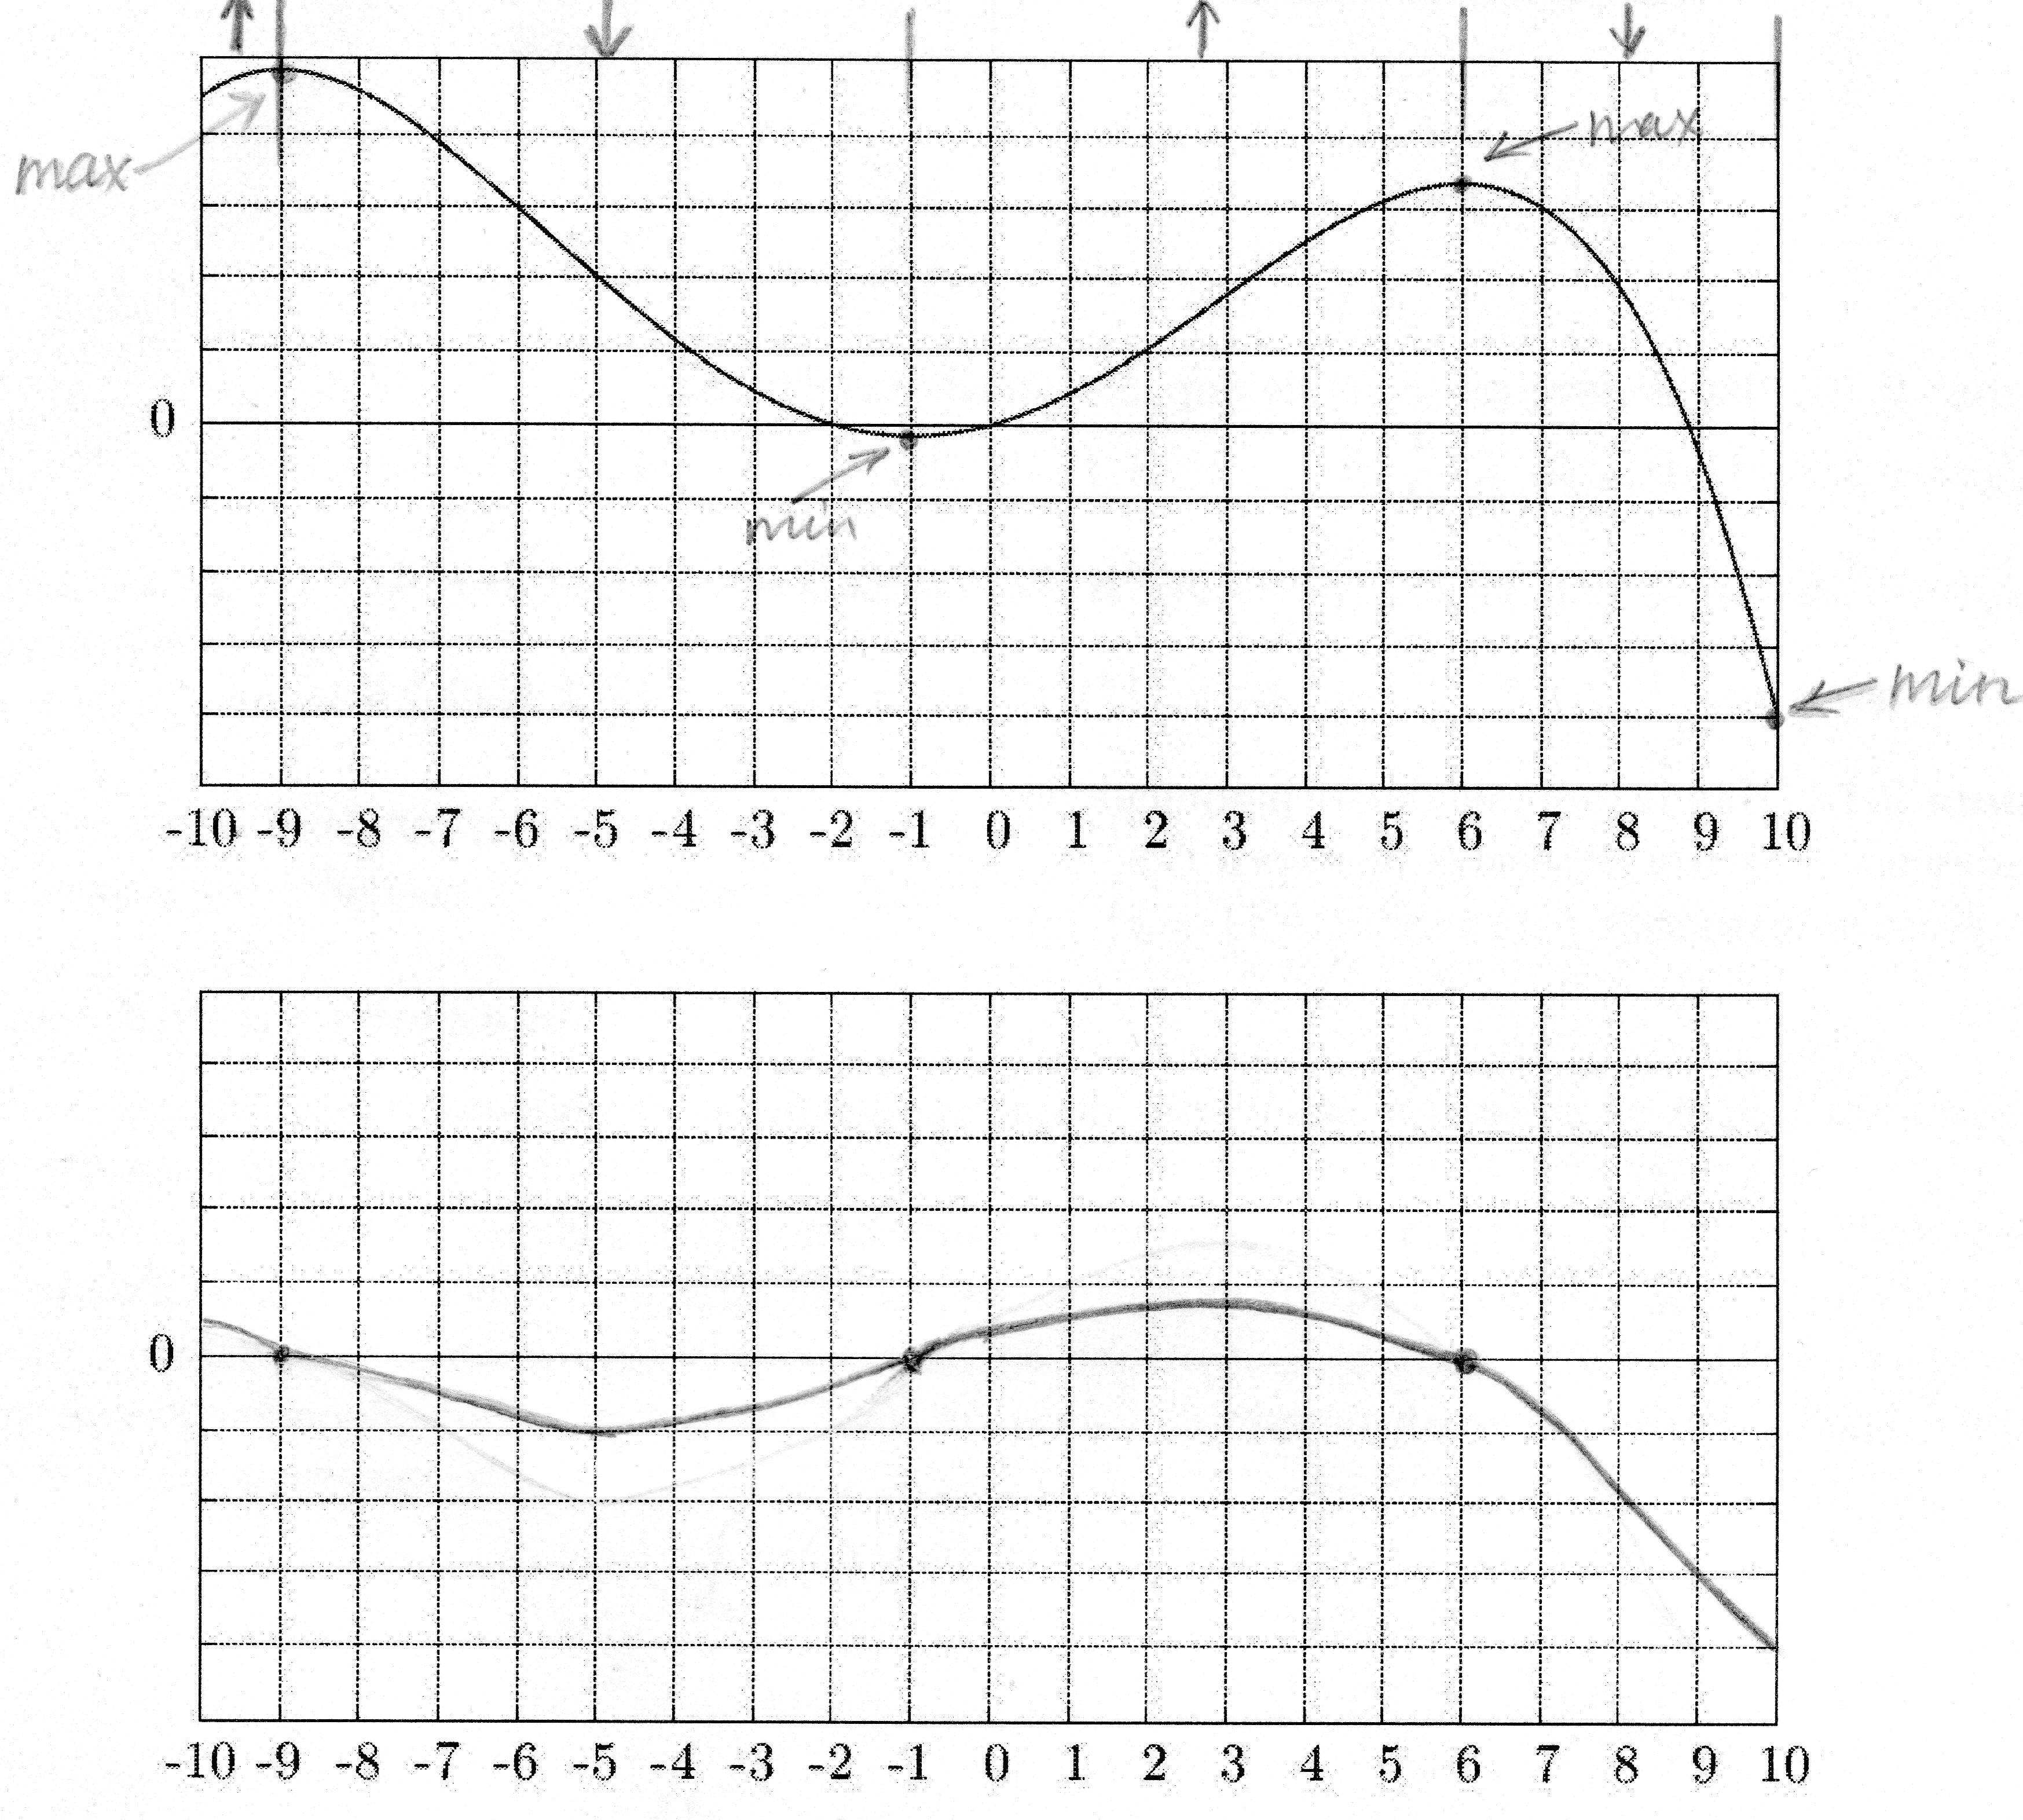
\includegraphics[scale=0.7]{images/task2a.jpg}
  \caption{График производной по графику её функции (пункт а)}
  \label{fig:task2a}
\end{figure}

\begin{figure}[h!]
  \centering
    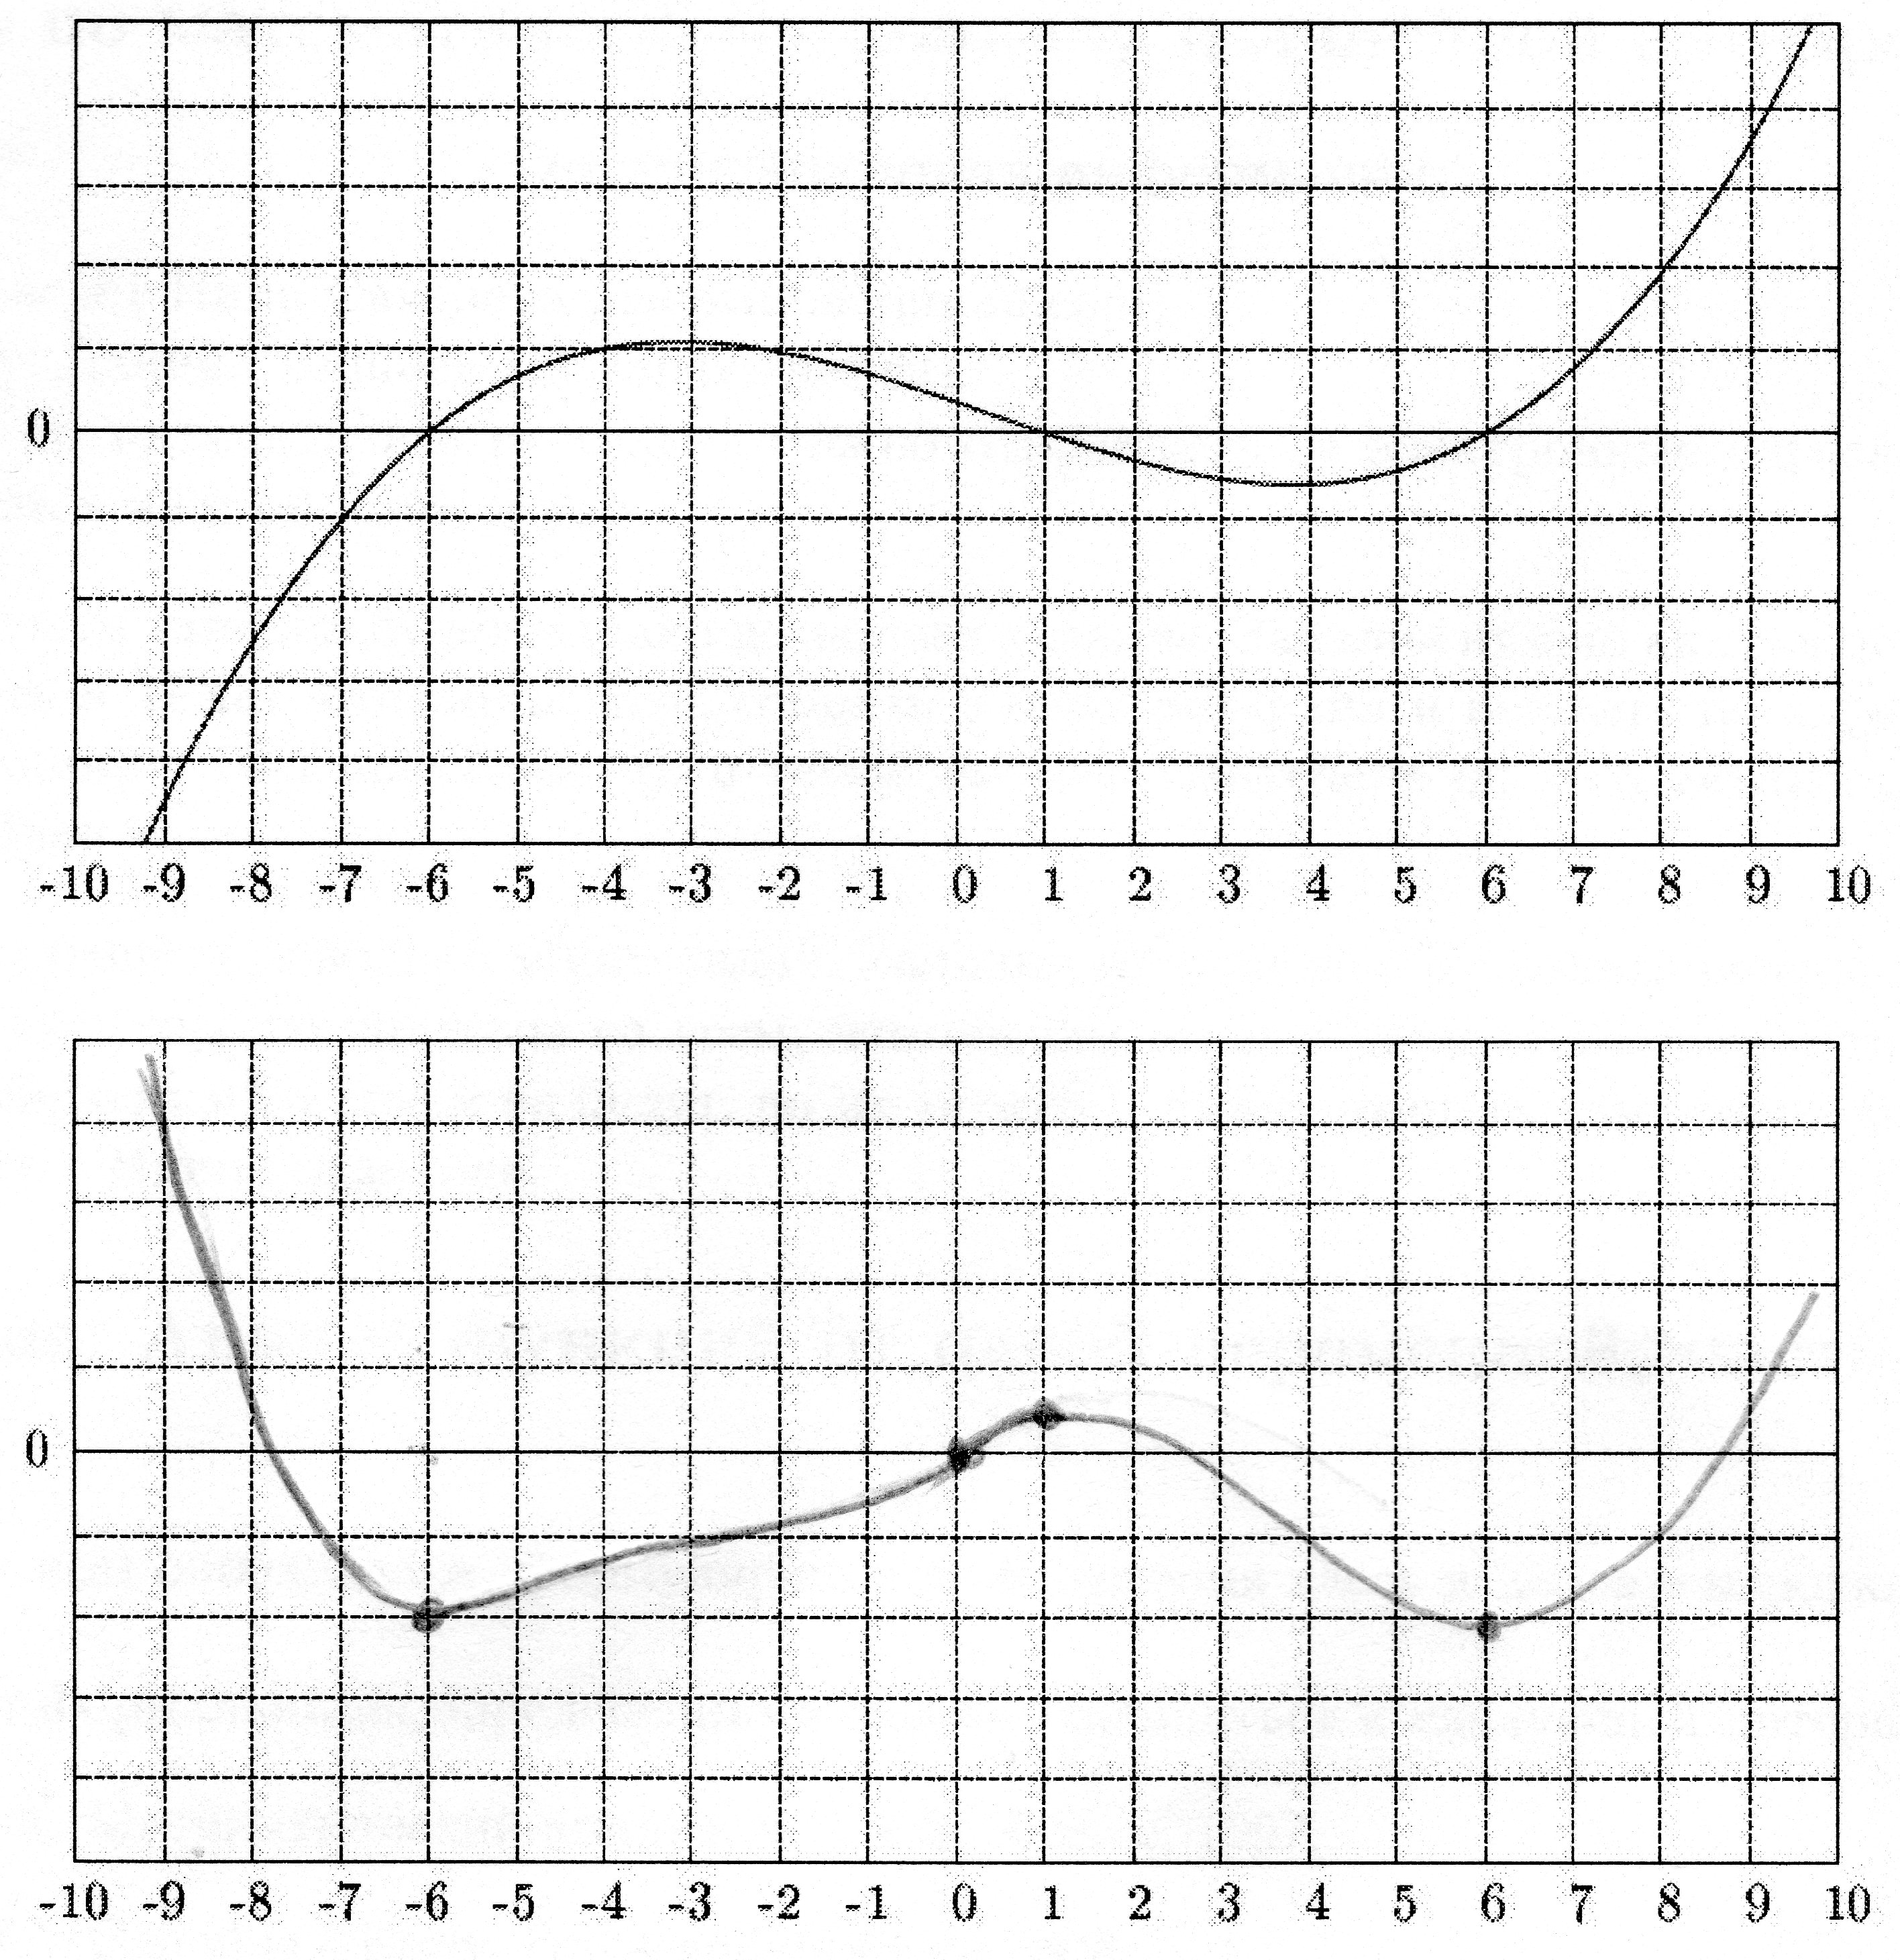
\includegraphics[scale=0.7]{images/task2b.jpg}
  \caption{График функции по графику её производной (пункт б)}
  \label{fig:task2b}
\end{figure}

\subsection{Задача 3}

Данная задача была выполнена в задаче 6 домашней работы 1.

\subsection{Задача 4}

1) данный пункт был выполнен в задаче 7 домашней работы 1,\\
2) данный пункт был выполнен в задаче 7 домашней работы 1,\\
3) не выполнен.

\subsection{Задача 5}

(не выполнена)

\subsection{Задача 6}

Попробуем оценить сходимость ряда, сравнив его с другим, с известной сходимостью. Обозначим, что заданный ряд - это $S_1 = \sum_{n=0}^{+\infty}\frac{1}{n!}$, он состоит из членов $a_n = \frac{1}{n!}$. Тогда, мы может его сравнить с рядом $S_2$ с членами $b_n = \frac{1}{2^n}$. Т.к. соблюдается условие, что $b_n > a_n, n \geq 4$, и $(a_1 + a_2 + a_3)$ - конечная сумма, то нам достаточно доказать, что ряд $S_2$ сходится. Несложно заметить, что $b_n$ - это члены геометрической прогрессии с $q = \frac{1}{2}$, сумма такого ряда равна $\frac{1}{1-q} = 2$. Т.к. данная сумма - конечна, то $S_2$ - сходится, соответственно, сходится и исходный ряд тоже сходится.

\subsection{Задача 7}

Воспользуемся теоремой Тейлора и найдём аппроксимацию значения функции в окрестности указанного значения аргумента функции. Положим $x_0$ равным нулю, учтём, что все производные любого порядка от $e^x$ равны $[e^x]^{(n)} = e^x$.  тогда:

\begin{align*}
e^x & = \sum_{i=0}^{n} \frac{x^i}{i!} \quad + \quad \frac{e^x}{(n+1)!}, |x -0| < 1 \\
\Rightarrow
e^{\sfrac{1}/{4}} & = \sum_{i=0}^{n} \frac{(\sfrac{1}{4})^i}{i!} \quad + \quad \frac{e^{\sfrac{1}{4}}}{(n+1)!}.
\end{align*}

Для оценки значения $n$ воспользуемся тем соображением, что остаточный член должен быть не больше требуемой погрешности 0.001:

\begin{align*}
\frac{e^{\sfrac{1}{4}}}{(n+1)!} \leq 0.001.
\end{align*}

Для разрешения данного неравенства воспользуемся каким-нибудь известным значением, ограничивающее значение в левой части неравенства сверху, при этом связанным с $n$, например,

\begin{align*}
\frac{e^{\sfrac{1}{4}}}{(n+1)!} < \frac{e^{\sfrac{1}{2}}}{(n+1)!} \leq 0.001.
\end{align*}

Значение $e^{\sfrac{1}{2}} \approx 1.7$, тогда методом подбора $n$ равно 6, т.е. достаточно вычислить сумму нулевого и остальных шести членов ряда, чтобы определить значение $e^{\sfrac{1}{4}}$ с точностью, не хуже заданной:

\begin{align*}
e^{\sfrac{1}{4}} \approx \sum_{i=0}^{6} \frac{(\sfrac{1}{4})^i}{i!} \approx 1.284.
\end{align*}

Значение суммы выше было вычислено на компьютере, используя программу, приведенную ниже. Также, были вычислены суммы и для других $n$, расположенных рядом. Любопытно отметить, что было бы достаточным взять $n=3$ для достижения требуемой точности.

\begin{lstlisting}[language=Python, caption=Python-скрипт для приближенного вычисления $e^{\sfrac{1}{4}}$]
import math

y = math.e**(1/4)

print('True:  y = %1.10f' % y)

print()

for n in (3,4,5,6):
    s = 0
    for i in range(n+1):
        s += (1/4)**i/math.factorial(i)
    print('n = %d, s = %1.10f, delta = %0.10f' % (n, s, abs(s - y)))
\end{lstlisting}

\vspace{0.5cm}

Вывод программы:

\begin{verbatim}
True:  y = 1.2840254167

n = 3, s = 1.2838541667, delta = 0.0001712500
n = 4, s = 1.2840169271, delta = 0.0000084896
n = 5, s = 1.2840250651, delta = 0.0000003516
n = 6, s = 1.2840254042, delta = 0.0000000125
\end{verbatim}

\subsection{Задача 8}

Представим заданную площадь $S$ на рис. \ref{fig:task8}. 

\begin{figure}[h!]
  \begin{center}
  \begin{tikzpicture}
  \begin{axis}[
      % only scale the axis, not the axis including the ticks and labels
      scale only axis=true,
      axis lines=middle,
      samples=100,
      % set `width' and `height' to the desired values
      width=8cm,
      height=6cm,
      xlabel = $x$,
      ylabel = $y$,
      xmin=-0.5, xmax=2.5,
      ymin=-0.5, ymax=1.5,
      %xtick={0,10,20,30,40,50,60}, 
      %ytick={0,0.5,1},
      %xmajorgrids=true,
      %ymajorgrids=true,
      %grid style=dashed,
      axis on top
    ]
    \addplot [
        name path=L1,
        domain=-1:3,
        color=green,
        line width=2pt
    ] {x^3};
    \addlegendentry{$x^3$}    
    \addplot [
        name path=L2,
        domain=0:3, 
        color=red,
        line width=2pt
    ] {1/x};
    \addlegendentry{$\frac{1}{x}$} 
    \addplot [
        name path=L3,
        domain=-1:3, 
        color=blue,
        line width=2pt
    ] {0};
    \addlegendentry{$y = 0$}
    \addplot +[
        name path=L4,
        color=orange,
        line width=2pt] 
    coordinates {(2, -1) (2, 3)};
    \addlegendentry{$x = 2$}
    % \addplot [yellow!50] fill between [of=L1 and L2];
    \node at (axis cs:1.25,0.25) {$S$};
    \draw [dashed] (1,0) -- (1,1);
  \end{axis}
  \end{tikzpicture}
  \end{center}
  \caption{Площадь заданная функциями}
  \label{fig:task8}
\end{figure}

Можно заметить, что она состоит из двух частей, разделённых линией $x^3 = \frac{1}{x}, x > 0 \Rightarrow x = 1$, соответственно, исходя из графиков функций, которые ограничивают её сверху, мы можем вычислить значение полной площади:

\begin{align*}
S = \int_{0}^{1} x^3 \,dx + \int_{1}^{2} \frac{1}{x} \,dx 
= \frac{1}{4} x^4 \bigg\vert_0^1 \quad + \quad \ln |x| \bigg\vert_1^2 
= \frac{1}{4} + \ln 2.
\end{align*}

\end{document}
